%Master File:lectures.tex


\lesson{Bayesian Inference}
\vspace{-1cm}
\begin{center}
  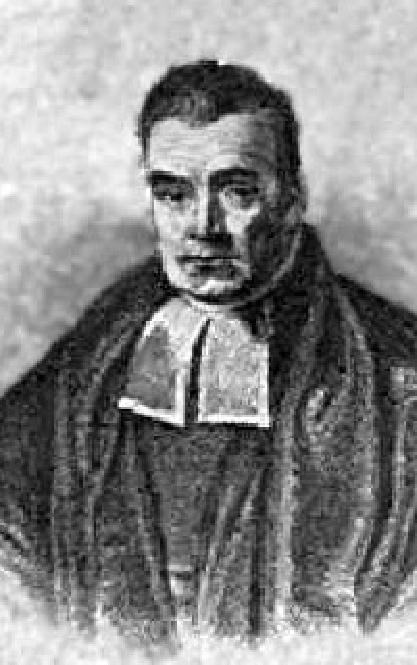
\includegraphics[height=10cm]{BayesPortrait}
\end{center}
\keywords{Bayes, Conjugate Priors, Uninformative Priors}
%%%%%%%%%%%%%%%%%%%%%%% Next Slide %%%%%%%%%%%%%%%%%%%%%%%
\renewcommand{\Outline}{%
\begin{slide}
\section[1]{Outline}

\begin{minipage}{10cm}\raggedright
  \begin{enumerate}\squeeze
    \outlineitem{Bayes' Rule}{bayes}
    \outlineitem{Conjugate Priors}{conjugatepriors}
    \outlineitem{Uninformative Priors}{applications}
  \end{enumerate}
\end{minipage}\hfill
\begin{minipage}{12cm}
  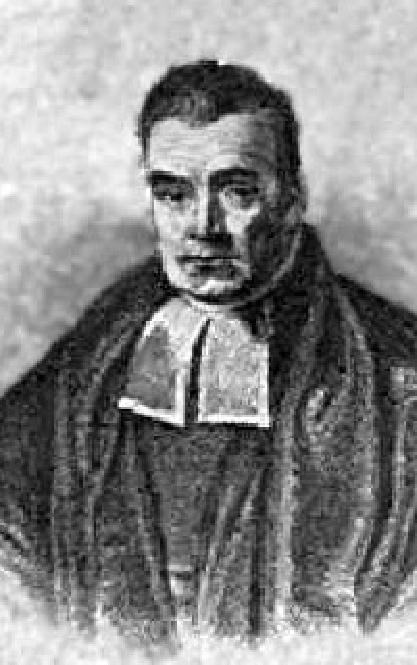
\includegraphics[height=14cm]{BayesPortrait}
\end{minipage}
\end{slide}
\addtocounter{outlineitem}{1}
}

\setcounter{outlineitem}{1}
\Outline % Motivation
\toptarget{firstoutline}
%%%%%%%%%%%%%%%%%%%%%%% Next Slide %%%%%%%%%%%%%%%%%%%%%%%

\begin{slide}
\section{Dealing with Uncertainty}

\begin{PauseHighLight}
  \begin{itemize}
  \item In machine learning we are attempting to make inference under
    uncertainty\pause 
  \item The natural language for discussing uncertainty is
    probability\pause
  \item The natural framework for making inferences is Bayesian
    statistics\pause
  \item However, this requires that we encode our prior knowledge of the
    problem\pause
  \item In consequence, probabilistic methods tend to be bespoke, rather
    then general purpose black boxes\pause
  \end{itemize}
\end{PauseHighLight}

\end{slide}

%%%%%%%%%%%%%%%%%%%%%%% Next Slide %%%%%%%%%%%%%%%%%%%%%%%

\begin{slide}
\section[-2]{Revision on Bayes}

\begin{PauseHighLight}

\begin{itemize}
\item  Bayes' rule
\begin{align*}
\pauselevel{=1, =2}\Prob{\hypo_i|\data}\pause\pauselevel{=1} =\pause
  \frac{\pauselevel{=1, =3}\Prob{\data|\hypo_i}\pause\,\pauselevel{=1, =4}\Prob{\hypo_i}\pause}{\pauselevel{=1, =5}\Prob{\data}}\pause
\end{align*}
\begin{itemize}\pauselevel{=2}
\item{$\Prob{\hypo_i|\data}$} is the \emph{posterior} probability of a
  hypothesis $\hypo_i$ (i.e.\ the probability of $\hypo_i$ \emph{after}
  we see the data)\pause\pauselevel{=3}
\item{$\Prob{\data|\hypo_i}$} is the \emph{likelihood} of the data given
  the hypothesis.  Note, that we calculated this from the forward
  problem\pause\pauselevel{=4}
\item{$\Prob{\hypo_i}$} is the \emph{prior} probability (i.e.\ the
  probability of $\hypo_i$ \emph{before} we see the data)\pause
  \pauselevel{=5}
\item{$\Prob{\data}$} is the \emph{evidence}\pause{} or \emph{marginal
    likelihood}\pauseb
  \begin{align*}
    \Prob{\data} = \sum_{i=1}^n\Prob{\hypo_i,\data}\pause
    = \sum_{i=1}^n \Prob{\data|\hypo_i} \,\Prob{\hypo_i}\pause
  \end{align*}
\end{itemize}
\end{itemize}

\end{PauseHighLight}
\end{slide}


%%%%%%%%%%%%%%%%%%%%%%% Next Slide %%%%%%%%%%%%%%%%%%%%%%%

\begin{slide}
\section[-1]{Solving Inverse Problems}

\begin{PauseHighLight}

\begin{center}
  \includegraphics[width=0.6\linewidth]{crystallography.png}
\end{center}
\begin{itemize}\squeeze
\item We want the posterior $\Prob{\hypo_i|\data}$ (i.e. the probability of
  what happened given some evidence)\pause
\item The Bayesian formalism converts this into the forward problem
\begin{align*}
\Prob{\hypo_i|\data} = \frac{\Prob{\data|\hypo_i}\,\Prob{\hypo_i}}{\Prob{\data}}\pause
\end{align*}
\end{itemize}

\end{PauseHighLight}
\end{slide}

%%%%%%%%%%%%%%%%%%%%%%% Next Slide %%%%%%%%%%%%%%%%%%%%%%%

\begin{slide}
\section{Bayesian Inference}

\begin{PauseHighLight}
  \begin{itemize}
  \item Bayes' rule says $\Prob{\hypo_i|\data} =
    \frac{\Prob{\data|\hypo_i}\,\Prob{\hypo_i}}{\Prob{\data}}$\pause
  \item We calculate the likelihood $\Prob{\data|\hypo_i}$ (i.e. assuming the
    hypothesis, what is the chance of obtaining the data?)\pause
  \item We consider the process of how the data is generated\pause
  \item This uses the data we have (doesn't care about missing data)\pause
  \item But we also need to know the prior $\Prob{\hypo_i}$\pause
  \item Also, this can get difficult when we have many hypotheses\pause
  \end{itemize}
\end{PauseHighLight}

\end{slide}


%%%%%%%%%%%%%%%%%%%%%%% Next Slide %%%%%%%%%%%%%%%%%%%%%%%

\begin{slide}
\section{Probability Density}

\begin{PauseHighLight}
  \begin{itemize}
  \item When we are working with continuous variables it is more natural
    to work with probability densities
    \begin{align*}
      f_X(x) = \lim_{\delta x \rightarrow 0} \frac{\Prob{x\leq X < x +
      \delta x}}{\delta x}\pause
    \end{align*}
  \item Note that densities are non-negative, but can be greater than
    1 (they are not probabilities)\pause
  \item However
    \begin{align*}
      \Prob{a\leq X \leq b} = \int_a^b f_X(x)\, \dd x
    \end{align*}
  is a probability and is less than or equal to 1\pause
  \end{itemize}
\end{PauseHighLight}

\end{slide}

%%%%%%%%%%%%%%%%%%%%%%% Next Slide %%%%%%%%%%%%%%%%%%%%%%%

\begin{slide}
\section[-2]{Densities and Bayes}

\begin{PauseHighLight}\squeeze
  \begin{itemize}
  \item Bayes' rule also applies to densities
    {\small \begin{align*}
      \Prob{x\leq X < x +\delta x| Y} = \frac{\Prob{Y | x} \,
      \Prob{x\leq X < x +\delta x}}{\Prob{Y}}\pause
    \end{align*}}
  \item Dividing by $\delta x$ and taking the limit $\delta x\rightarrow
    0$
    {\small \begin{align*}
      f_{X|Y}(x|Y) = \frac{\Prob{Y|x}\,f_X(x)}{\Prob{Y}}\pause
    \end{align*}}
  \item Similarly if $X$ is discrete and $Y$ continuous
    {\small \begin{align*}
      \Prob{X|y} = \frac{f_{Y|X}(y|X)\,\Prob{X}}{f_Y(y)}\pause
    \end{align*}}
  \item If both $X$ and $Y$ are continuous
    {\small \begin{align*}
      f_{X|Y}(x|Y) = \frac{f_{Y|X}(y|x)\,f_X(x)}{f_Y(y)}\pause
    \end{align*}}
  \end{itemize}
\end{PauseHighLight}
\end{slide}

%%%%%%%%%%%%%%%%%%%%%%% Next Slide %%%%%%%%%%%%%%%%%%%%%%%

\begin{slide}
\section{Practical Bayesian Inference}
 
\begin{PauseHighLight}
  \begin{itemize}
  \item Often consider learning parameters $\bm{\theta}$
    \begin{align*}
      p(\bm{\theta}|\data) =
      \frac{p(\data|\bm{\theta})\,p(\bm{\theta})}{p(\data)}\pause
    \end{align*}
  \item This can be hard for large data sets as the posterior,
    $p(\bm{\theta}|\data)$ is a mess\pause
  \item If we are lucky and have a simple likelihood then if we choose
    the right prior we end up with a posterior of the same form as the
    prior\pause
  \item This occurs in some classic probabilistic inference problems,
    but as we will see soon it is also true for Gaussian Processes\pause
  \end{itemize}
\end{PauseHighLight}

\end{slide}



%%%%%%%%%%%%%%%%%%%%%%% Next Slide %%%%%%%%%%%%%%%%%%%%%%%
\Outline % Simple Example
%%%%%%%%%%%%%%%%%%%%%%% Next Slide %%%%%%%%%%%%%%%%%%%%%%%

\begin{slide}
\section[-1]{Learning a Probability}

\begin{PauseHighLight}
  \begin{itemize}
  \item Suppose we have a coin and we want to establish the probability
    of a head\pause
  \item We want to learn this from a series of independent trials\pause
  \item (Independent trials with two possible outcomes are known in
    probability theory as Bernoulli trials)\pause
  \item Let $X_i$ equal 1 if the $i^{th}$ trial is a head and 0
    otherwise\pause 
  \item If the probability of a head is $p$ then the \emph{likelihood}
    of a $X_i$ is
    \begin{align*}
      \Prob{X_i|p} = p^{X_i} (1-p)^{1-X_i}\pause =
      \begin{cases}
        p & \text{if $X_i=1$}\\
        (1-p) & \text{if $X_i=0$}
      \end{cases}\pauseb
    \end{align*}
  \end{itemize}
\end{PauseHighLight}

\end{slide}


%%%%%%%%%%%%%%%%%%%%%%% Next Slide %%%%%%%%%%%%%%%%%%%%%%%

\begin{slide}
\section[-2]{Prior}

\begin{PauseHighLight}
  \begin{itemize}
  \item We may have a prior belief (e.g. we have made a few trials or
    we see the coin looks like a normal penny)\pause
  \item We will suppose we can model our prior belief in terms of a\\
    \emph{Beta distribution}
    \begin{align*}
      f(p) = \mathrm{Beta}(p|a,b) = \frac{p^{a-1}(1-p)^{b-1}}{B(a,b)}\pause
    \end{align*}
  \item $B(a,b)$ is just a normalisation constant
    \begin{align*}
      B(a,b) = \int_0^1 p^{a-1}(1-p)^{b-1} \dd p =
      \frac{\Gamma(a)\,\Gamma(b)}{\Gamma(a+b)} \pause
    \end{align*}
  \item This is a useful function for modelling the distribution of a
    random variable in the range 0 to 1\pause
  \end{itemize}
\end{PauseHighLight}

\end{slide}

%%%%%%%%%%%%%%%%%%%%%%% Next Slide %%%%%%%%%%%%%%%%%%%%%%%

\begin{slide}
\section{Uninformative Prior}

\begin{PauseHighLight}
  \begin{itemize}
  \item Suppose we have no idea about $p$ what should we do?\pause
  \item Laplace (one of the first Bayesian's) suggested giving equal
    weighting to all values of $p$\pause
  \item This corresponds to a beta distribution with $a=b=1$\pause
  \item (Surprisingly other arguments suggest using $a=b=0$ which
    provides a strong bias towards $p=0$ and $p=1$)\pause
  \item Given enough data the prior is not so important and we will
    stick with Laplace for now\pause
  \end{itemize}
\end{PauseHighLight}

\end{slide}


%%%%%%%%%%%%%%%%%%%%%%% Next Slide %%%%%%%%%%%%%%%%%%%%%%%

\begin{slide}
\section[-2]{Independent Trials}

\begin{PauseHighLight}
  \begin{itemize}
  \item Using Bayes' rule
    \begin{align*}
      f(p|\data) &= \frac{ \Prob{\data| p}\, f(p) }{ \Prob{\data} }\pause
    \end{align*}
  \item Assuming the trials are independent (a reasonably fair
    assumption for tossing coins) then the likelihood factorises
    \begin{align*}
      \Prob{\data| p} &= \prod_{i=1}^n p^{X_i} (1-p)^{1-X_i}\pause
      \\
      &= p^{X_1} (1-p)^{1-X_1} p^{X_2} (1-p)^{1-X_2}
      \cdots p^{X_n} (1-p)^{1-X_n}\pause
      \\
      &= p^{\sum_i X_i} (1-p)^{\sum_i (1-X_i)} = p^s (1-p)^{n-s}
    \end{align*}
    $s = \sum_i X_i$ (number of successes/heads)\pause
  \end{itemize}
\end{PauseHighLight}

\end{slide}

%%%%%%%%%%%%%%%%%%%%%%% Next Slide %%%%%%%%%%%%%%%%%%%%%%%

\begin{slide}
\section{Posterior}

\begin{PauseHighLight}
  \begin{itemize}
  \item Plugging in a prior $f(p) = \mathrm{Beta}(p|a_0,b_0)$
    \begin{align*}
      f(p|\data) &= 
      \frac{ \Prob{\data| p}\, f(p) }{ \Prob{\data} }
      = \frac{p^s (1-p)^{n-s}  \times p^{a_0-1} (1-p)^{b_0-1} }{
                   \Prob{\data} \, B(a_0,b_0) }\pause
    \end{align*}
  \item The denominator is a normalising factor
    \begin{align*}
     \hspace{-1cm} \Prob{\data} &= \int_0^1  \Prob{\data| p}\, f(p) \, \dd p =
      \int_0^1 \frac{p^{s+a_0-1} (1-p)^{n-s+b_0-1}}{B(a_0,b_0)} \dd p \\
      &= \frac{B(s+a_0,n-s+b_0)}{B(a_0,b_0)}\pause
    \end{align*}
  \end{itemize}
\end{PauseHighLight}

\end{slide}

%%%%%%%%%%%%%%%%%%%%%%% Next Slide %%%%%%%%%%%%%%%%%%%%%%%

\begin{slide}
\section[-2]{Conjugate Priors}

\begin{PauseHighLight}
  \begin{itemize}
  \item The posterior distribution is Beta distribution
    \begin{align*}
      f(p|\data) &= 
      \frac{p^{s+a_0-1} (1-p)^{n-s+b_0-1}}{B(s+a_0,n-s+b_0)} =
                   \mathrm{Beta}(p|s+a_0,n-s+b_0)\pause
    \end{align*}
  \item Something rather nice happened\pause
  \item Starting with a beta distributed prior
    $f(p) = \mathrm{Beta}(p|a_0,b_0)$ for a set of Bernoulli trials we
    obtain a beta distributed posterior
    $f(p|\data) = \mathrm{Beta}(p| a_0+s, b_0+n-s)$\pause
  \item This is not always the case (often the posterior will be very
    complicated) but it happens for a few likelihoods and priors\pause
  \item When the posterior is the same as the prior then the likelihood
    and prior distributions are said to be \emph{conjugate}\pause
  \end{itemize}
\end{PauseHighLight}

\end{slide}


%%%%%%%%%%%%%%%%%%%%%%% Next Slide %%%%%%%%%%%%%%%%%%%%%%%

\begin{slide}
\section[-2]{Incremental Updating}

\begin{PauseHighLight}
  \begin{itemize}
  \item For independent data we can update incrementally $\data = (X_1,
    X_2, \ldots, X_n)$
    \begin{align*}
      f(p|X_1) &= \frac{\Prob{X_1|p} f(p)}{\Prob{X_1}} \pause
      \\
      f(p|X_1,X_2) &= \frac{\Prob{X_2|p} f(p|X_1)}{\Prob{X_2}} \pause
      \\ 
      \vdots \quad &= \quad \vdots
      \\
      f(p|X_1,X_2,\ldots, X_n) &= \frac{\Prob{X_n|p} 
        f(p|X_1,\ldots,X_{n-1})}{\Prob{X_n}}\pause
    \end{align*} 
  \item The posterior becomes the prior for the next piece of data\pause
  \item For our problem the posterior is always Beta distributed\pause
  \end{itemize}
\end{PauseHighLight}

\end{slide}

%%%%%%%%%%%%%%%%%%%%%%% Next Slide %%%%%%%%%%%%%%%%%%%%%%%

\begin{slide}
\section[-1]{Example (p=0.7)}
\pb
\pause\pauselevel{=1}
\begin{center}
  \multipdf[width=0.9\linewidth]{bernoulliTrials}\pause
\end{center}
\end{slide}

%%%%%%%%%%%%%%%%%%%%%%% Next Slide %%%%%%%%%%%%%%%%%%%%%%%

\begin{slide}
\section{Estimating Prediction Errors}

\begin{PauseHighLight}
  \begin{itemize}
  \item A full Bayesian treatment gives a prediction of its own
    error\pause
  \item Assuming $f(p|\data) = \mathrm{Beta}(p|a,b)$
  \item The expected value of $p$ is given by $a/(a+b) = 23/32 = 0.719$\pause
  \item The standard deviation is
    \begin{align*}
      \sqrt{\frac{a\,b}{(a+b)^2(a+b+1)}} = 0.078\pause
    \end{align*}
  \end{itemize}
\end{PauseHighLight}

\end{slide}
%%%%%%%%%%%%%%%%%%%%%%% Next Slide %%%%%%%%%%%%%%%%%%%%%%%

\begin{slide}
\section{Poisson Likelihoods}

\begin{PauseHighLight}
  \begin{itemize}
  \item Let's look at a second example of conjugate priors\pause
  \item Suppose we want to find the rate of traffic along a road between
    1:00pm and 2:00pm\pause
  \item We assume the number of cars is given by a Poisson distribution
    \begin{align*}
      \Prob{N} = \mathrm{Pois}(N|\mu) = \frac{\mu^N}{N!} \e{-\mu}\pause
    \end{align*}
  \item $\mu$ is the rate of traffic per hour which we want to infer
    from observation taken on different days\pause
  \end{itemize}
\end{PauseHighLight}

\end{slide}

%%%%%%%%%%%%%%%%%%%%%%% Next Slide %%%%%%%%%%%%%%%%%%%%%%%

\begin{slide}
\section{Using Bayes}

\begin{PauseHighLight}
  \begin{itemize}
  \item Let us assume a Gamma distributed prior
    \begin{align*}
      p(\mu) = \Gamma(\mu|a_0,b_0) =
      \frac{b_0^{a_0}\, \mu^{a_0-1} \e{-b_0\,\mu}}{\Gamma(a)}\pause
    \end{align*}
  \item We will assume that we know nothing.  The uninformative prior is
    $a_0=b_0=0$\pause
  \item The data is $\data=\{N_1, N_2, \ldots, N_n\}$\pause
  \item The likelihood is $\mathrm{Pois}(N_i|\mu)$\pause
  \end{itemize}
\end{PauseHighLight}

\end{slide}

%%%%%%%%%%%%%%%%%%%%%%% Next Slide %%%%%%%%%%%%%%%%%%%%%%%

\begin{slide}
\section{Posterior}

\begin{PauseHighLight}
  \begin{itemize}
  \item The posterior after seeing the first piece of data is
    \begin{align*}
      p(\mu|N_1) &\propto \Prob{N_1|\mu}\, p(\mu) \pause
      \\
      &\propto \frac{\mu^{N_1}}{N_1!} \e{-\mu} \, \mu^{a_0-1} \e{-b_0\,\mu}
      \\
      &\propto \mu^{N_1+a_0-1} \e{-(b_0+1)\mu}\pause
    \end{align*}
  \item The posterior is also a Gamma distribution
    $\Gamma(\mu|a_1,b_1)$ with $a_1=a_0+N_1$, $b_1=b_0+1$\pause
  \end{itemize}
\end{PauseHighLight}

\end{slide}

%%%%%%%%%%%%%%%%%%%%%%% Next Slide %%%%%%%%%%%%%%%%%%%%%%%

\begin{slide}
\section[-2]{Example ($\mu=5$)}
\pb
\pause\pauselevel{=1}
\begin{center}
  \multipdf[width=\linewidth]{inferGamma}\pause
\end{center}
\vspace*{-1cm}
\begin{align*}
  \av{\mu} &= \frac{a}{b} = \frac{96}{20} = 4.8 &
  \sqrt{\Var{\mu}} &=  \sqrt{\frac{a}{b^2}} = 0.49\pause
\end{align*}
\end{slide}

%%%%%%%%%%%%%%%%%%%%%%% Next Slide %%%%%%%%%%%%%%%%%%%%%%%
\Outline
%%%%%%%%%%%%%%%%%%%%%%% Next Slide %%%%%%%%%%%%%%%%%%%%%%%

\begin{slide}
\section{Uninformative Priors}

\begin{PauseHighLight}
  \begin{itemize}
  \item What if we have no prior knowledge, what should we do?\pause
  \item OK usually we know whether we should make a measurement using a
    micrometer, ruler or car mileage, but we might still know almost
    nothing\pause
  \item This led to Bayesian statistics being labelled as
    \textit{subjective}\pause
  \item However Ed. Jaynes (the greatest proponent of Bayesian methods)
    argued that we could answer this using symmetry arguments\pause
  \end{itemize}
\end{PauseHighLight}

\end{slide}


%%%%%%%%%%%%%%%%%%%%%%% Next Slide %%%%%%%%%%%%%%%%%%%%%%%

\begin{slide}
\section[-3]{Uninformative Priors for Scale Parameter}

\pb
\begin{itemize}\pause\pauselevel{=1}
\item Why did we choose $a_0=b_0=0$ implying a prior
  $p(\mu)=1/\mu$?\pauseh\pauselevel{=1}
  \begin{center}
    \multipdf[width=0.6\linewidth]{scaleParameter}\pause
  \end{center}
\item That is, we have no idea on what scale to measure $\mu$
  \begin{align*}
    \int_A^B p(\mu) \, \dd \mu = \int_{A/c}^{B/c} p(\mu) \, \dd \mu\pauseh
    = \int_A^B \frac{1}{c} \, p(\frac{\nu}{c}) \,\dd \nu\pauseb
    = \int_A^B \frac{1}{c} \, p(\frac{\mu}{c}) \,\dd \mu\pauseb
  \end{align*}
  making a change of variables $\mu=\nu/c$\pauselevel{=6}\pauseb
\item Or $ p(\mu)= \frac{1}{c}\, p(\frac{\mu}{c})$ implying
  $p(\mu)\propto \frac{1}{\mu}$\pauseh
\end{itemize}

\end{slide}

%%%%%%%%%%%%%%%%%%%%%%% Next Slide %%%%%%%%%%%%%%%%%%%%%%%

\begin{slide}
\section{Benford's Law}

\begin{PauseHighLight}
  \begin{itemize}
  \item Numbers occurring in life (physical constants, amounts of money)
    should not depend on the units (scale) measuring them\pause
  \item They should then be distributed as $p(x) \propto 1/x$\pause
  \item A curious consequence of this is that the significant figure has
    a distribution
    \begin{align*}
      \Prob{\mbox{most s.f. of $x=n$}} &= \frac{ \int_n^{n+1} \frac{1}{x} \,
        \dd \, x}{\int_1^{10} \frac{1}{x} \,
        \dd \, x}\pause = \frac{ \int_{10\,n}^{10\,n+10} \frac{1}{x} \,
        \dd \, x}{\int_{10}^{100} \frac{1}{x} \,
        \dd \, x}\pauseb
      \\
      &=  \frac{\logg{n+1}-\logg{n}}{\logg{10}} =
      \log_{10}\!\left(\frac{n+1}{n}\right)\pause
    \end{align*}
  \end{itemize}
\end{PauseHighLight}

\end{slide}

%%%%%%%%%%%%%%%%%%%%%%% Next Slide %%%%%%%%%%%%%%%%%%%%%%%

\begin{slide}
\section[-2]{Population Size of 238 Countries}

\begin{center}
  \includegraphics[width=0.9\linewidth]{BenfordPop}\\
  Significant Figure
\end{center}
\end{slide}

%%%%%%%%%%%%%%%%%%%%%%% Next Slide %%%%%%%%%%%%%%%%%%%%%%%

\begin{slide}
\section[-1]{Conclusion}

\begin{PauseHighLight}
  \begin{itemize}
  \item Bayesian inference provides a coherent framework which we can
    use for machine learning\pause
  \item However, it requires a model of what is happening\pause
  \item In practice Bayesian methods are easy if the data is generated
    from a likelihood with a conjugate prior distribution---we have to
    be clever to choose the right prior\pause
  \item We will see in the next lecture that much more frequently we
    will have likelihoods with no conjugate prior and we have to work
    much harder\pause
  \item When we have no knowledge there are consistent ways to express
    our ignorance\pause
  \end{itemize}
\end{PauseHighLight}

\end{slide}


%%% Local Variables:
%%% TeX-master: "lectures"
%%% End:
